\section{对数 GLSM（Qile Chen）}%
\label{sec:Log GLSM (Qile Chen)}

设 \(X\) 为光滑射影簇（甚至是 DM叠）。设 \(E\) 为 \(X\) 上的向量丛，带有一个截面 \(s \in H^0(E)\)，它在预期的余维数上定义了一个光滑的零截面 \(Z\)。我们将 \(X\) 和 \(E\) 称为环境（ambient），将 \(s\) 和 \(Z\) 称为完全交。

\begin{quest}
    \(Z\) 的 GW 理论与 \((X, E)\) 的 GW 理论之间有何关系？
\end{quest}

当 \(g = 0\) 时，Givental 与 Lian-Liu-Yau 利用这一关系计算了完全交的 GW 不变量，而当 \(g = 1\) 时，这由 Zinger 完成。一般而言，有两种方法：(N)MSP 与对数 GLSM。在本系列讲座中，我们将讨论对数 GLSM。\footnote{若听众对 MSP 有疑问，Qile 让他们咨询这些笔记的作者以及 Yang Zhou。}

\subsection{R-映射}%
\label{sub:R-maps}

我们将考虑 \textit{R-环面} \(\C^{\times}_{\omega} \coloneqq \C^{\times}\)。它有一个权重为 \(1\) 的表示，我们称之为 \(\C_{\omega}\)。它下降为线丛 \(\mc{L}_{\omega} \coloneqq [\C_{\omega} / \C^{\times}_{\omega}]\)，位于 \(B \C_{\omega}^{\times}\) 上。R-映射的目标将是叠
\[ \P \to B \C^{\times}_{\omega} \]
它们是 DM 型、分离且（对数）光滑的。现在，一个 R-映射由如下 (2-)交换图构成
\begin{equation*}
\begin{tikzcd}
    & \mf{P} \ar{d} \\
    C \ar{ur}{f} \ar{r}[swap]{\omega^{\log}} \ar{d} & B \C_{\omega}^{\times} \\
    S.
\end{tikzcd}
\end{equation*}
这里，曲线可以是预稳定的、扭的、对数的，甚至是穿孔的。

\begin{exm}
    我们的第一个例子是稳定映射。设 \(\mf{P} = B\C_{\omega}^{\times}\)。因为在图
    \begin{equation*}
    \begin{tikzcd}
        & X \times B\C_{\omega}^{\times} \ar{d} \\
        C \ar{ur} \ar{r} & B \C_{\omega}^{\times}
    \end{tikzcd}
    \end{equation*}
    中竖直箭头是第二投影，我们看到它约化为到 \(X\) 的映射。
\end{exm}

\begin{exm}
    考虑映射
    \begin{equation*}
    \begin{tikzcd}
        & \mc{L}_{\omega} \ar{d} \\
        C \ar{ur}{f} \ar{r} & B \C_{\omega}^{\times}.
    \end{tikzcd}
    \end{equation*}
    若假设 \(C\) 无标记点，我们看到这个映射的数据仅仅是 \(\omega_C\) 的一个截面，因此我们恢复了全纯微分。
\end{exm}

\begin{exm}
    考虑一个态射 \(\C^{\times}_R \to \C^{\times}_{\omega}\)，它由 \(z \mapsto z^{r_{\mr{in}}}\) 给出。于是我们看到
    \[ \mc{L}_R^{\otimes r_{\mr{in}}} \simeq \mc{L}_{\omega} |_{B \C_R^{\times}}. \]
    现在一个带有无标记点 \(C\) 的图
    \begin{equation*}
    \begin{tikzcd}
        & B \C_R^{\times} \ar{d} \\
        C \ar{ur}{f} \ar{r} & B \C_{\omega}^{\times}
    \end{tikzcd}
    \end{equation*}
    等价于一个线丛 \(\mc{L}_R|_C\) 以及一个同构 \(\mc{L}_R^{\otimes r_{\mr{in}}} \simeq \omega_C\) 的数据。或者，我们可以考虑形如
    \begin{equation*}
    \begin{tikzcd}
        & \mc{L}_R \ar{d} \\
        & B \C_R^{\times} \ar{d} \\
        C \ar{uur}{f} \ar{r} & B \C_{\omega}^{\times},
    \end{tikzcd}
    \end{equation*}
    的 R-映射，它们参数化带有 R-spin 线丛以及一个截面的曲线。
\end{exm}

\begin{exm}
    设 \(X\) 为光滑射影簇。则考虑形如
    \begin{equation*}
    \begin{tikzcd}
        & E^{\vee} \boxtimes \mc{L}_{\omega} \ar{d} \\
        & X \times B \C_{\omega}^{\times} \ar{d} \\
        C \ar{uur}{f} \ar{r} & B \C_{\omega}^{\times}.
    \end{tikzcd}
    \end{equation*}
    的 R-映射。这等价于一个映射 \(C \to X\) 连同截面 \(\rho \in H^0(E^{\vee}|_C \otimes \omega_C)\)。
\end{exm}

我们将考虑 GW 情形中的目标。
考虑环境 \((X, E)\) 的数据。则我们将设 \(\mf{P}^{\circ} \coloneqq E^{\vee} \boxtimes \mc{L}_{\omega}\)。态射 \(\mf{P}^{\circ} \to B \C_{\omega}^{\times}\) 非常好，但它不是真的。为修正这一点，我们将考虑对数叠
\[ \mf{P} = ( \P(E^{\vee} \boxtimes \mc{L}_{\omega} \oplus \mc{O}) , \infty). \]
因为我们在光滑叠中有一个光滑除子，映射 \(\mf{P} \to B \C_{\omega}^{\times}\) 是真且对数光滑的。注意到我们有零截面
\[ 0_{\mf{P}} \subset \mf{P}^{\circ} \subset \mf{P} \supset \infty. \]

我们现在考虑 r-spin 情形中的目标。考虑对数叠
\[ (\P(\mc{L}_R^{\oplus n} \oplus \mc{O}), \infty) = \mf{P} \to B \C_R^{\times} \to B \C_{\omega}^{\times}. \]
这个态射是真且对数光滑的。

\subsection{对数 R-映射与穿孔 R-映射}%
\label{sub:Log and punctured R-maps}

我们将考虑图
\begin{equation*}
\begin{tikzcd}
    & \mf{P} \ar{d} \\
    C \ar{ur}{f} \ar{r}[swap]{\omega^{\log}} \ar{d} & B \C_{\omega}^{\times} \\
    S
\end{tikzcd}
\end{equation*}
其中 \(C \to S\) 是一条对数曲线或穿孔（可能扭）曲线，而 \(S\) 是 fs 对数概形。GW 情形中的稳定性条件是 \(f\) 可表且
\[ (\omega_{\log})^{1+\delta} + H^{\otimes k} \otimes f^* \mc{O}(\infty) > 0 \]
对所有 \(0 < \delta \ll 1\) 与 \(k \gg 1\) 成立，其中 \(H\) 是 \(X\) 的粗模空间上的丰富线丛。对于穿孔 R-映射，我们进一步要求预稳定性。

\begin{exm}
    考虑全纯微分的情形。则考虑 \(f \in H^0(\omega_C)\)，使得所有零点都集中在单个 Weierstrass 点，其中 \(C\) 的亏格为 \(2\)。若我们考虑 \(\lim_{\lambda \to \infty} \lambda \cdot f\)，则极限由一个亏格 \(2\) 分支（它完全映射到 \(\infty\)）以及一个记住该零点的有理分支组成。
\end{exm}

我们现在讨论对数 R-映射或穿孔 R-映射的热带化。回顾一个图
\[ \ul{G} = (\V, \H, \imath \colon \H \to \H, v \colon \H \to \V) \]
由顶点集 \(\V\)、半边集 \(\H\)、半边上的对合 \(\imath\)，以及一个从半边到顶点的根映射组成。然后我们记腿集 \(\L\) 为
\[ \L = \ab\{ h \in \H \mid \imath(h) = h\}. \]
边是对合将之互相映射的不同半边的对：
\[ \E = \ab\{ \ab\{h, \hat{h}\} \mid \imath(h) = \hat{h} \neq h \}. \]
现在一个装饰图是一个图连同亏格函数
\[ g \colon \V \to \N, \]
一个赋值
\[ r \colon \H \to \N, \]
以及一个排序
\[ m \colon \L \to \ab\{0, \ldots, n\}. \]

\begin{exm}
    \leavevmode\par
    \begin{center}
    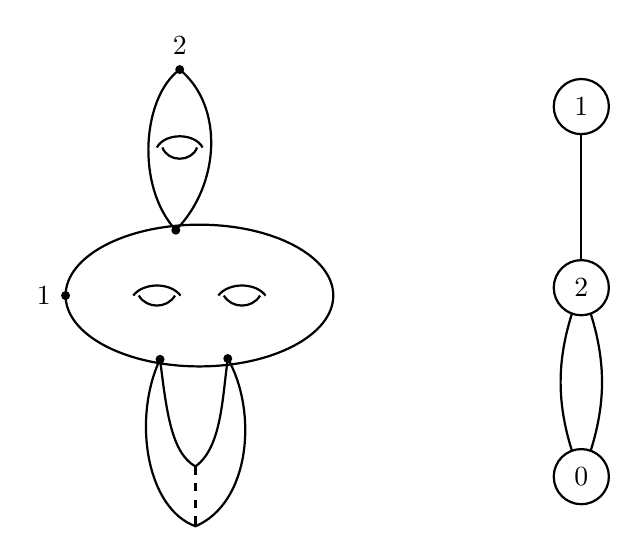
\begin{tikzpicture}[
        x=1cm,
        y=1cm,
        curve component/.style={thick},
        marked point/.style={circle,fill=black,inner sep=1.15pt},
        graph vertex/.style={
            circle,draw,thick,fill=white,minimum size=7mm,inner sep=0pt
        }
    ]
        % A three-component curve with components of genera 1, 2, and 0.
        \draw[curve component] (1.5,3.65) ellipse [x radius=1.7,y radius=0.9];

        % The two handles on the genus-two component.
        \draw[curve component]
            (0.66,3.65)
            .. controls (0.79,3.82) and (1.13,3.82) .. (1.26,3.65);
        \draw[curve component]
            (0.73,3.65)
            .. controls (0.83,3.48) and (1.09,3.48) .. (1.19,3.65);
        \draw[curve component]
            (1.74,3.65)
            .. controls (1.87,3.82) and (2.21,3.82) .. (2.34,3.65);
        \draw[curve component]
            (1.81,3.65)
            .. controls (1.91,3.48) and (2.17,3.48) .. (2.27,3.65);

        % The genus-one component attached above.
        \coordinate (uppernode) at (1.2,4.48);
        \draw[curve component]
            (uppernode)
            .. controls (0.68,5.05) and (0.78,6.18) .. (1.25,6.52)
            .. controls (1.82,6.05) and (1.76,5.05) .. cycle;
        \draw[curve component]
            (0.96,5.53)
            .. controls (1.06,5.72) and (1.44,5.72) .. (1.54,5.53);
        \draw[curve component]
            (1.03,5.53)
            .. controls (1.10,5.34) and (1.40,5.34) .. (1.47,5.53);

        % The rational component attached at two nodes below.
        \coordinate (lowerleft) at (1.00,2.84);
        \coordinate (lowerright) at (1.86,2.85);
        \draw[curve component]
            (lowerleft)
            .. controls (0.65,2.10) and (0.82,0.95) .. (1.45,0.72)
            .. controls (2.15,1.02) and (2.24,2.18) .. (lowerright);
        \draw[curve component]
            (lowerleft)
            .. controls (1.08,2.20) and (1.14,1.65) .. (1.45,1.48)
            .. controls (1.78,1.72) and (1.79,2.34) .. (lowerright);
        \draw[curve component,dashed] (1.45,1.48) -- (1.45,0.72);

        % Nodes and marked points.
        \node[marked point] at (uppernode) {};
        \node[marked point] at (lowerleft) {};
        \node[marked point] at (lowerright) {};
        \node[marked point,label=left:{$1$}] at (-0.2,3.65) {};
        \node[marked point,label=above:{$2$}] at (1.25,6.52) {};

        % The dual graph: the vertex labels record the genera.
        \coordinate (vone) at (6.35,6.05);
        \coordinate (vtwo) at (6.35,3.75);
        \coordinate (vzero) at (6.35,1.35);
        \draw[curve component] (vone) -- (vtwo);
        \draw[curve component]
            (vtwo) to[out=-112,in=112] (vzero);
        \draw[curve component]
            (vtwo) to[out=-68,in=68] (vzero);
        \node[graph vertex] at (vone) {$1$};
        \node[graph vertex] at (vtwo) {$2$};
        \node[graph vertex] at (vzero) {$0$};
    \end{tikzpicture}
    \end{center}
\end{exm}

对于一个对数 R-映射或穿孔 R-映射
\begin{equation*}
\begin{tikzcd}
    & \mf{P} \ar{d} \\
    C \ar{ur}{f} \ar{d} \ar{r} & B \C_{\omega}^{\times} \\
    S,
\end{tikzcd}
\end{equation*}
我们将通过对整个图取相伴的广义锥复形来热带化它。因为 \(B \C_{\omega}^{\times}\) 没有对数结构，我们看到的是
\begin{equation*}
\begin{tikzcd}
    \Sigma(C) \ar{d} \ar{r}{\Sigma(f)} & \Sigma(\mf{P}) = \R_{\geq 0} \\
    \Sigma(S).
\end{tikzcd}
\end{equation*}
现在设 \(S = \Spec (Q \to \C)\) 是一个对数点，其中 \(Q\) 是 fs 尖幺半群。特别地，这意味着 \(\Sigma(S) = Q_{\R}^{\vee}\)。因为一切是（分片）线性的，只需考虑内点 \(t \in \Sigma(S)\) 并考虑 \(\Sigma(C)_t\)。

对于每条半边，我们将其视为从所附顶点向外指向，特别地，这意味着到 \(\R_{\geq 0}\) 的线性映射对应于一个斜率。我们称这些为 \textit{接触阶}。特别地，我们有 \(c(h) = - c(\hat{h})\)，若 \(h \neq \hat{h}\) 由 \(\imath\) 相关联。对所有 \(v \in \V\)，我们还定义 \textit{退化}（degeneracy）
\[ e_v \colon Q_{\R}^{\vee} \to \R_{\geq 0} \qquad t \mapsto \Sigma(f)_t (v). \]
特别地，\(e_v \in Q\) 是一个整点。

接下来我们需要引入的是穿孔腿。它们将记为
\[ \L^{\circ} = \ab\{ h \in \H \mid \Sigma(f)_t(h) \text{ is bounded and nontrivial for all } t \in Q_{\R}^{\vee}\}. \] 
我们将在 \(h \in \L^{\circ}\) 处定义预稳定性，使得 \(0 \in \ol{\Sigma(f)_t(h)}\)，这是一个技术上必需的假设。在所有穿孔腿都预稳定的假设下，我们可以定义 \textit{边长度}函数
\[ \ell \colon \E \cup \L^{\circ} \to \ms{Map}(Q_{\R}^{\vee}, \R_{\geq 0}) \qquad x \mapsto \ell(x) \colon t \mapsto \ell(x)(t). \]
注意到 \(\ell(E) \in Q\) 对于边 \(E\) 也是一个整点。对于穿孔腿，这在细分意义下成立。

